\documentclass{szzclass}

\title{Vzory používané během návrhu: třívrstvá architektura, Model View Controller, GoF vzory (Abstraktní továrna, Stav, Adaptér).}
\author{Jakub Rathouský}

\begin{document}
\maketitle
\newpage
\tableofcontents
\newpage

\section{Třívrstvá architektura}
Vhodná pro složitější (enterprise) aplikace, vrstvy:
\begin{itemize}
    \item Prezentační
    \item Business (doménová)
    \item Datová (technické služby)
\end{itemize}

Rozděluje se na dva typy:
\begin{itemize}
    \item striktní - závislost vždy směrem dolů a pouze o jednu úroveň
    \item relaxovaná - závislost vždy směrem dolů, přes libovolný počet úrovní, nejvíce používaná
\end{itemize}
\subsection{Prezentační vrstva}
\begin{itemize}
    \item obsahuje HTML stránky, šablony, třídy pro zpracování požadavků uživatelů, navigace mezi stránkami\dots
    \item poskytují GUI, API
    \item problém závislosti zdola nahoru
\end{itemize}
\subsection{Business vsrtva}
\begin{itemize}
    \item business logika
    \item procesy a validace
    \item nezávislá na prezentační vrstvě a datové vrstvě
\end{itemize}
\subsection{Datová vrstva}
\begin{itemize}
    \item persistence dat
\end{itemize}
\subsection{Výhoda třívrstvé architektury}
\begin{itemize}
    \item oddělení business logiky od prezentační vrstvy
    \item nezávislost business logiky na způsobu uložení
    \item snadná výměna jednotlivých vrstev
    \item jednoduché testování
    \item více různých prezentačních vrstev
    \item znovu použitelnost
    \begin{itemize}
        \item čím nižší vrstva tím víc je možné jí znovu použít (logování, persistence, odesílání emailů\dots)
        \item čím vyšší vrstva, tím je specifičtější pro konkrétní projekt
    \end{itemize}
\end{itemize}
\section{Model View Controller (MVC)}
Vzor řešící problém prezentační vrstvy. Založený na oddělení logiky od GUI. Třívrstvá architektura.
\begin{itemize}
    \item model
    \item view
    \item controller - zpracovává uživatelský vstup
\end{itemize}
Rozděluje se na dva typy modelu:
\begin{itemize}
    \item aktivní - upozorňuje na změny, které nastaly
    \item pasivní - pouze reaguje na požadavky
\end{itemize}
Jedná se velmi často o součást existujících řešení:
\begin{itemize}
    \item Spring MVC
    \item Swing
    \item React, Angular
    \item \dots
\end{itemize} 
\subsection{Model View Presenter (MVP)}
Podobná verze MVC. Událost odchytí View, ale zpracování deleguje na Presenter. GUI založené na komponentách.
\begin{itemize}
    \item model
    \item view - zpracovává uživatelský vstup
    \item presenter
\end{itemize}

\section{GoF vzory}
Rozdělení:
\begin{itemize}
    \item vzory pro vytváření objektů (creational)
    \begin{itemize}
        \item abstraktní továrna (abstract factory)
        \item stavitel (builder)
    \end{itemize}
    \item strukturální vzory (structural)
    \begin{itemize}
        \item adaptér (adapter)
    \end{itemize}
    \item vzory chování (behavioral)
    \begin{itemize}
        \item stav (state)
        \item pozorovatel (observer)
    \end{itemize}
\end{itemize}
\subsection{Abstraktní továrna (Abstract factory)}
\begin{itemize}
    \item poskytuje rozhraní pro vytváření skupiny objektů bez znalosti konkrétní implementace
    \item konkrétní implementace je dána použitou továrnou
\end{itemize}
\begin{figure}[h!]
    \includegraphics[width=0.95\textwidth]{topics/bi-wsi-si-19/images/abstractFactory.png}
    % \includegraphics[width=0.95\textwidth]{images/abstractFactory.png}
\end{figure}
\subsection{Stavitel (Builder)}
\begin{itemize}
    \item director - řídí strukturu výsledného produktu
    \item builder
    \begin{itemize}
        \item umít postavit jednotlivé části produktu v konkrétní technologii
        \item je řízen Directorem
    \end{itemize}
\end{itemize}
\begin{figure}[h!]
    \includegraphics[width=0.95\textwidth]{topics/bi-wsi-si-19/images/builder.png}
    % \includegraphics[width=0.95\textwidth]{images/builder.png}
\end{figure}
\newpage
\subsection{Stav (State)}
\begin{itemize}
    \item odděluje chování třídy závislé na stavu do samostatné třídy
    \item odstraňuje složité větvení (switch, case, if, else)
    \item libovolný počet stavů
    \item snadné přidání nového stavu
\end{itemize}
\begin{figure}[h!]
    \includegraphics[width=0.95\textwidth]{topics/bi-wsi-si-19/images/state.png}
    % \includegraphics[width=0.95\textwidth]{images/state.png}
\end{figure}
\subsection{Pozorovatel (Observer)}
\begin{itemize}
    \item pozorující objekty se zaregistrují u pozorovaného objektu
    \item pozorující objekt musí implementovat požadované rozhraní
    \item při změně upozorní pozorovaný objekt všechny pozorující pomocí tohoto rozhraní
\end{itemize}
\begin{figure}[h!]
    \includegraphics[width=0.95\textwidth]{topics/bi-wsi-si-19/images/observer.png}
    % \includegraphics[width=0.95\textwidth]{images/observer.png}
\end{figure}
\subsection{Adaptér (Adapter)}
\begin{itemize}
    \item konvertuje rozhraní jedné třídy na rozhraní jiné
    \item umožňuje propojit třídy s ruzným rozhraním
\end{itemize}
\begin{figure}[h!]
    \includegraphics[width=0.95\textwidth]{topics/bi-wsi-si-19/images/adapter.png}
    % \includegraphics[width=0.95\textwidth]{images/adapter.png}
\end{figure}
\end{document}